%%%%%%%%%%%%%%%%%%%%%%%%%%%%%%%%%%%%%%%%%
% Journal Article
% LaTeX Template
% Version 1.3 (9/9/13)
%
% This template has been downloaded from:
% http://www.LaTeXTemplates.com
%
% Original author:
% Frits Wenneker (http://www.howtotex.com)
%
% License:
% CC BY-NC-SA 3.0 (http://creativecommons.org/licenses/by-nc-sa/3.0/)
%
%%%%%%%%%%%%%%%%%%%%%%%%%%%%%%%%%%%%%%%%%

%----------------------------------------------------------------------------------------
%	PACKAGES AND OTHER DOCUMENT CONFIGURATIONS
%----------------------------------------------------------------------------------------

\documentclass[twoside]{article}

\usepackage{lipsum} % Package to generate dummy text throughout this template


\usepackage[sc]{mathpazo} % Use the Palatino font
\usepackage[T1]{fontenc} % Use 8-bit encoding that has 256 glyphs
\usepackage[utf8]{inputenc}
\linespread{1.05} % Line spacing - Palatino needs more space between lines
\usepackage{microtype} % Slightly tweak font spacing for aesthetics
\usepackage{amsmath}
\usepackage{listings}

\lstset{
    basicstyle=\ttfamily\footnotesize,
    breaklines=true
}


%\usepackage[hmarginratio=1:1,top=32mm,columnsep=20pt]{geometry} % Document margins
\usepackage[margin={1cm,2cm}]{geometry}
\setlength{\columnsep}{1cm}
\usepackage{multicol} % Used for the two-column layout of the document
\usepackage[hang, small,labelfont=bf,up,textfont=it,up]{caption} % Custom captions under/above floats in tables or figures
\usepackage{booktabs} % Horizontal rules in tables
\usepackage{float} % Required for tables and figures in the multi-column environment - they need to be placed in specific locations with the [H] (e.g. \begin{table}[H])
\usepackage{hyperref} % For hyperlinks in the PDF
\usepackage{multirow}

\usepackage{syntax}
\setlength{\grammarparsep}{5pt plus 1pt minus 1pt} % increase separation between rules
\setlength{\grammarindent}{6em} % increase separation between LHS/RHS 

\usepackage{lettrine} % The lettrine is the first enlarged letter at the beginning of the text
\usepackage{paralist} % Used for the compactitem environment which makes bullet points with less space between them

\usepackage{abstract} % Allows abstract customization
\renewcommand{\abstractnamefont}{\normalfont\bfseries} % Set the "Abstract" text to bold
\renewcommand{\abstracttextfont}{\normalfont\small\itshape} % Set the abstract itself to small italic text


\usepackage{graphicx}

\usepackage{pgf}
\usepackage{tikz}
\usetikzlibrary{arrows,automata, shapes, positioning, calc}

\newcommand{\rparen}{)}

\usepackage{titlesec} % Allows customization of titles
\renewcommand\thesection{\Roman{section}} % Roman numerals for the sections
%\renewcommand{\thesubsection}{\thesection\hspace{1mm}\alph{subsection}}
\titleformat{\section}[block]{\large\scshape\centering}{\thesection}{1em}{} % Change the look of the section titles
\titleformat{\subsection}[block]{\large}{\thesubsection}{1em}{} % Change the look of the section titles

\usepackage{fancyhdr} % Headers and footers
\pagestyle{fancy} % All pages have headers and footers
\fancyhead{} % Blank out the default header
\fancyfoot{} % Blank out the default footer
\fancyhead[C]{IT3708 Sub-symbolic AI Methods $\bullet$ Project 2 $\bullet$ \date{\today}} % Custom header text
\fancyfoot[RO,LE]{\thepage} % Custom footer text

%----------------------------------------------------------------------------------------
%	TITLE SECTION
%----------------------------------------------------------------------------------------

\title{\vspace{-15mm}\fontsize{18pt}{10pt}\selectfont\textbf{Programming an Evolutionary Algorithm - Project Report}} % Article title

\author{
    \large
    \textsc{Øyvind Robertsen} \\ % Your name
    \normalsize Norwegian University of Science \& Technology \\ % Your institution
    \normalsize \href{mailto:oyvinrob@stud.ntnu.no}{oyvinrob@stud.ntnu.no} % Your email address
    \vspace{-5mm}
}
\date{}

%----------------------------------------------------------------------------------------

\begin{document}

\maketitle % Insert title

\thispagestyle{fancy} % All pages have headers and footers

%----------------------------------------------------------------------------------------
%	ABSTRACT
%----------------------------------------------------------------------------------------

\begin{abstract}

\noindent This report describes a solution to Project 2 in the subject IT3708 at NTNU. 
The purpose of this project is to implement a basic evolutionary algorithm and use it to solve various problems.
Given a properly defined problem, an evolutionary algorithm searches for a solution by repeatedly evolving a population of possible solutions.
The algorithm applies a set of selection strategies and genetic operators on the population to gradually improve the quality of individuals with regards to the problem defenition.

\end{abstract}

%----------------------------------------------------------------------------------------
%	ARTICLE CONTENTS
%----------------------------------------------------------------------------------------

\begin{multicols}{2} % Two-column layout throughout the main article text

    \section{Implementation}

    I chose to implement my EA using the Python programming language.

    When using an EA to solve a problem, there are many parameters and settings to consider.
    Everything from population size to which genetic operators to use.
    Early on, I decided to make an attempt at separating concerns between what relates strictly to the problem definition, and what relates to this particular attempt at solving the problem.

    This separation led very naturally to separating my implementation into two distinct classes; the \texttt{EARunner} and the \texttt{Problem} classes.
    The \texttt{EARunner} class encapsulates the main evolutionary loop and all configurable parameters that are problem independent, but still important to configure for an EA run.
    The \texttt{Problem} class acts more like an interface (In that if it is instanced, most of the functions it defines will just raise an exception that will halt the program and tell the programmer he/she will need to provide an actual implementation of the function in question.) that the programmer will use as a blueprint when defining the problem they want to solve.
    
    In my implementation, a well-defined problem must include/implement the following:
    fitness assessment, initial population generation, genotype to phenotype conversion, genome component mutation function and genotype size.
    These are all parameters that in total define the problem we want to solve.
    They influence the process of evolution, but are aspects of the problem, not of a particular EA run attempting to solve it.

    Parameters that relate specifically to characteristics of a particular EA run are specified by instancing an \texttt{EARunner}.
    These include, among others, choices of adult and parent selection strategies, genetic operator choice and population size.
    I chose to allow users to specify total population size, adult and child individuals in total, and then also specify how big a portion of that total should be adults.
    Individuals are represented by the \texttt{Individual} class that encapsulates genotype, phenotype, fitness and maturity.
    The run is started by calling the \texttt{solve()} method of the configured \texttt{EARunner} instance.

    The two classes discussed so far are the main building blocks of my implementation.
    Additionaly, I've implemented a library of functions commonly used by EAs, e.g.: various parent and adult selection strategies, genetic mutators and crossover operators.
    I've also created a simple command line interface for simple testing of the problems I have implemented.
    When doing multiple runs and tweaking parameters, the CLI is cumbersome to use however, and it is significantly easier to write a startup script accompanying the problem definition.
    
    \subsection{Modularity and reusability}

    The most restricting assumptions that my implementation makes are the following:

    \begin{itemize}
        \item The initial population must be an iterable of \texttt{Individual}-instances
        \item A complete configuration for the \texttt{EARunner} instance, very few parameters are optional
    \end{itemize}

    As mentioned earlier, all problem specifics are encapsulated in the \texttt{Problem} subclass that the programmer will have to implement, making it very easy to introduce new geno-/phenotypes, genetic operators, etc.
    These operators would have to implement the same interface that the already existing functions do (e.g.: the parent selection function takes an iterable of individuals and \texttt{kwargs} as arguments, and returns an individual from the iterable).
    With regards to the library of functions I have implemented, they only make one assumption about the encoding of genotype/phenotype, namely that it is an iterable.

    As an example of how simple it is to extend the library, let's implement a new adult selection strategy.
    What we want to achieve is a hybrid strategy that fills half of the adult pool with randomly chosen individuals from the existing pool of adults, and the other half with the best children.
    The interface for the adult selection functions is: \texttt{population, **kwargs -> population}.


    \begin{lstlisting}[language=Python, caption=Adult selection, label={lst:adult-selection}]
    def hybrid_adult_selection(population, **kwargs):
        if kwargs['number_of_adults']:
            number_of_adults = kwargs.pop('number_of_adults')
        else:
            sys.exit('hybrid adult selection requires number of adults to be specified.')
        new_pop = random.sample(population, number_of_adults/2)
        children = sorted(list(filter(lambda ind: not ind.mature, population)), key=lambda ind: ind.fitness)
        while len(new_pop) < number_of_adults:
            new_pop.append(children.pop())
        return new_pop
    \end{lstlisting}

    To specify that this is the adult selection function we want to use, we would pass it as an argument to the EARunner instance.
    Any parameters that you need in an extension function that you implement yourself can be included via the keyword arguments of the \texttt{solve} method.
    

    \section{Performance on the One-Max problem}

    We want to look at the 40-bit One-Max problem, utilizing full generational replacement as an adult selection strategy and fitness proportionate parent selection. 
    The first order of business is to determine an approximate minimal population size for which the EA can consistently find a solution in under 100 generations.
    This was determined by gradually increasing population size until I reached a number for which ten out of ten runs managed to find an optimal solution.
    With the crossover and mutation rates I used (0.8 and 0.01, respectively), I needed a population of 600 to achieve this criteria.

    \subsection{Varying crossover and mutation}

    With a population of 600 individuals, we want to look at how the crossover rate and mutation rate parameters influence the search.
    Figure \ref{fig:one-max-varying-cr-mr} shows the average fitnesses through at most 100 generations with a population size of 600 individuals, full generational replacement adult selection, fitness proportionate parent selection and varying crossover and mutation rates. 
    Per genome mutation and one point crossover was used as genetic operators.


    \begin{figure}[H]
        \centering
        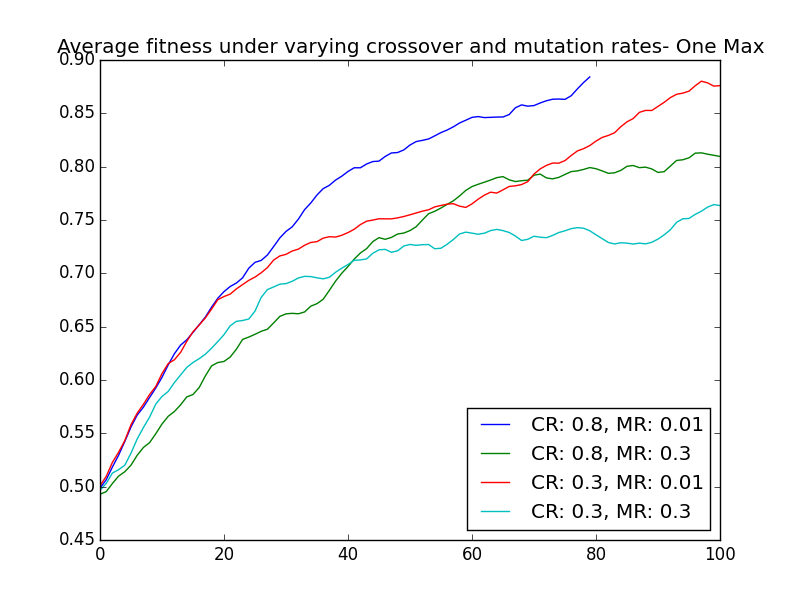
\includegraphics[width=\linewidth]{images/one-max-varying-cr-mr.png}
        \caption{Average fitness through 100 generations under varying crossover and mutation rates.} \label{fig:one-max-varying-cr-mr}
    \end{figure}

    As the graph shows, the values I initially used, high ($0.8$) crossover rate and low ($0.01$) mutation rate gives the highest efficiency.
    For the One Max problem specifically, this makes sense, since doing a lot of random mutations is likely to decrease the fitness of an individual, and recombining two good genotypes will in general have a low probability of resulting in an individual with lower fitness than it's predecessors.
    

    \subsection{Varying parent selection}

    Keeping the parameters we've found to be optimal so far, namely a population of 600, high crossover rate and low mutation rate, we now want to examine which parent selection strategy yields the best results.
    Figure \ref{fig:one-max-varying-parent-selection} shows the average fitnesses using four different parent selection strategies.
    
    The clear winners are sigma scaling and tournament selection.
    They both apply high (relative to fitness proportionate selection) selection pressure, ensuring that we retain/recombine high fitness genotypes.
    Boltzmann selection reduces selection pressure relative to fitness proportionate selection, which is useless since the fitness landscape has only one global maximum.


    \subsection{Random bitstring as ideal}

    Using the optimal parameters we've found so far, we want to know if the problem of finding a random 40-bit string is harder than finding a 40-bit string of all ones.
    My hypothesis is that since fitness landscape is the same (the one global maximum has just moved), the problem is no more difficult than the One Max problem.
    Figure \ref{fig:one-max-vs-random} shows the results of doing 50 runs with each of the problems, plotting the number of generations spent searching for each of the runs.
    The average is also calculated, giving us a clear indicator that the random problem is indeed no more difficult than the regular One Max problem.
    

    \begin{figure}[H]
        \centering
        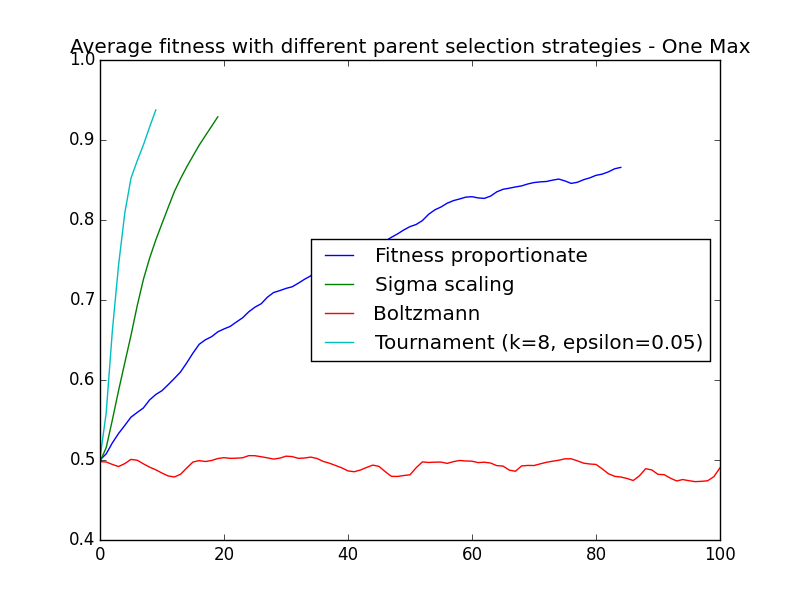
\includegraphics[width=\linewidth]{images/one-max-varying-parent-selection.png}
        \caption{Average fitness through 100 generations with different parent selection methods.} \label{fig:one-max-varying-parent-selection}
    \end{figure}


    \begin{figure}[H]
        \centering
        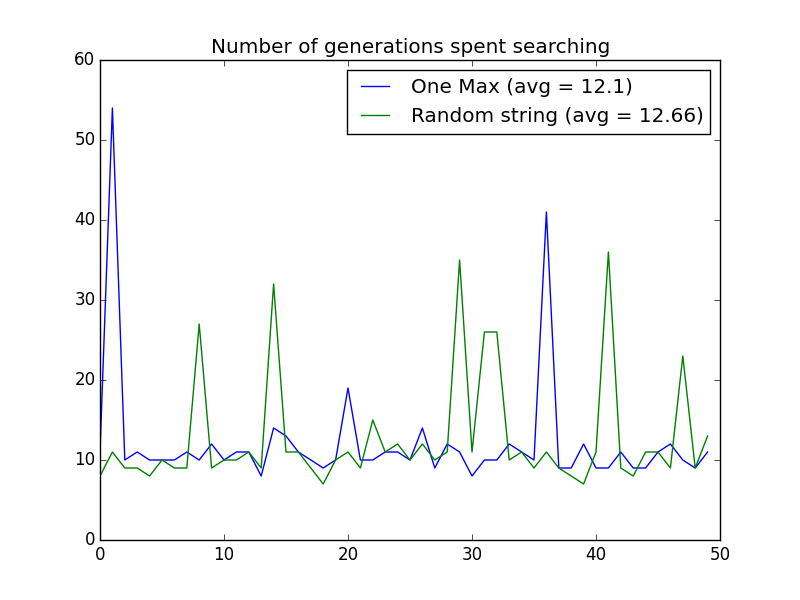
\includegraphics[width=\linewidth]{images/one-max-vs-random.png}
        \caption{Number of elapsed generations for 50 runs of both regular One Max and random bitstring} \label{fig:one-max-vs-random}
    \end{figure}


    \subsection{LOLZ behaviour}

    Figure \ref{fig:lolz-8-runs} shows the average fitness through at most 100 generations of eight separate runs of the LOLZ problem.
    The configuration used is the same as the optimal one discovered previously for the One Max problem.

    \begin{figure}[H]
        \centering
        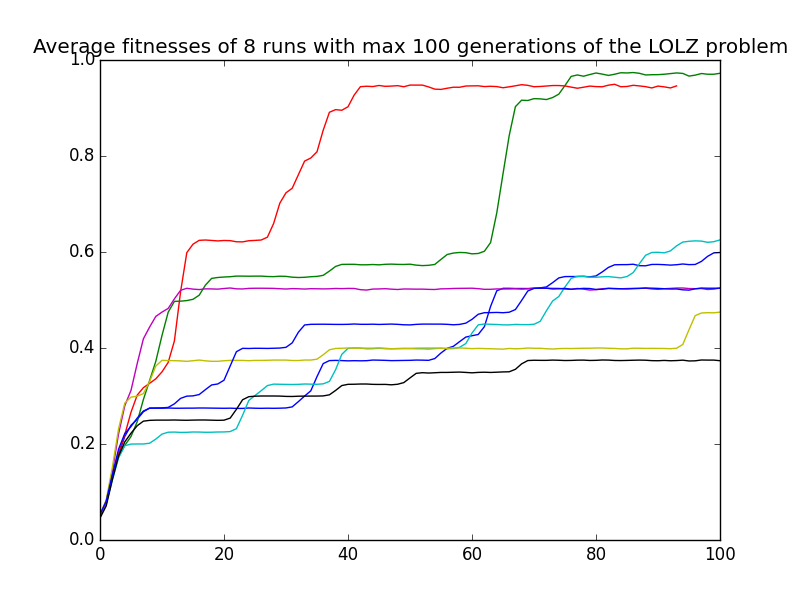
\includegraphics[width=\linewidth]{images/lolz-8-runs.png}
        \caption{Average fitness through 100 generations of 8 runs} \label{fig:lolz-8-runs}
    \end{figure}

    From the graph we see that two of the runs have managed to escape the danger of getting stuck in the local maxima of the "leading zero"-neighborhood, while the rest have not been as fortunate.


    \section{Surprising Sequences}

    \subsection{Encoding}
    
    To keep the implementation simple, I chose to encode the symbols as integers directly into the genotype.
    That is, a single genotype component is an integer representing a single symbol.
    The genotype-to-phenotype translation step therefore does nothing.
    (I contemplated drawing a useless figure illustrating this, but decided against in the interest of saving space.)

    \subsection{Fitness}

    The mathematics behind the fitness calculation for both globally and locally surprising sequences is simply $\frac{1}{1 + E}$, where $E$ is the number of violations for the phenotype in question.
    Counting violations differs for globally vs. locally surprising sequences.


    For locally surprising sequences this is done by iterating through the phenotype, maintaining a set of encountered pairs of symbols.
    At each step of the iteration, we look at the pair consisting of the current symbol and the subsequent one.
    If such a pair is already in the set of encountered symbols, the number of violations is incremented.
    Otherwise, we add the pair to the set.

    Globally surprising sequences are slightly more convoluted.
    A violation in the context of this problem is any reocurrence of a pair of symbols with a substring of some length between them.
    For example, if we find an ocurrence of symbol $A$, followed by three symbols, subsequently followed by symbol $B$, any other similar subsequence ($AX_{3}B$) is a violation.
    In practice, we perform the count by maintaining a set of encountered subsequences as we iterate through the phenotype.
    With locally surprising sequences it is enough to look at the current symbol and the subsequent one only.
    For globally surprising sequences, we have to look at all subsequences from the current symbol to the end of the phenotype.
    As with the local version, if an encountered subsequence is already in the set, we increment the violation count, if not, we add the subsequence to the set.

    With the fitness definition I have employed, the fitness landscape will be gradually more granular from a fitness value of $0.5$ and down.
    To illustrate, no violations result in a fitness of $1$, a single violation $0.5$, two violations $0.33$, etc.
    Since the EA makes no assumptions about the fitness landscape of the problem, this has no effect on the simulation.

    \subsection{Locally Surprising Sequences}

    \begin{table}[H]
        \centering
        \begin{tabular}{|l|l|l|}
            \hline
            $S$  & Genotype size & Generations \\ \hline
            3    & 10            & 0           \\ \hline
            5    & 26            & 85          \\ \hline
            10   & 100           & 378         \\ \hline
            15   & 220           & 2604        \\ \hline
            20   & 362           & 3219        \\ \hline
        \end{tabular}
    \end{table}

    Sequences omitted for sanity. (Are available in attached \texttt{local.txt} file.)
    Other parameters are: population size of 200, full generational replacement for adult selection, tournament selection($k=32$, $\epsilon = 0.05$) for parent selection, crossover rate at $0.8$ and mutation rate at $0.009$.


    \subsection{Globally Surprising Sequences}

    \begin{table}[H]
        \centering
        \begin{tabular}{|l|l|l|}
            \hline
            S  & Genotype size & Generations \\ \hline
            3  & 7             & 0           \\ \hline
            5  & 12            & 259         \\ \hline
            10 & 25            & 379         \\ \hline
            15 & 37            & 619         \\ \hline
            20 & 49            & 2113        \\ \hline
        \end{tabular}
    \end{table}

    Sequences attached in \texttt{global.txt}.
    Other parameters: population size 200, full replacement, tournament selection($k=64$, $\epsilon=0.05$), crossover rate $0.01$, mutation rate $0.01$.


    \section{Difficulty}

    From high difficulty to low, the ranking is as follows:

    \begin{enumerate}
        \item Globally surpising sequences
        \item Locally surprising sequences
        \item LOLZ
        \item One Max
    \end{enumerate}

    The One Max problem has a fitness landscape that is very easy for an EA to traverse.
    With only a single global maximum, if the EA applies some selection pressure, it is guaranteed to be moving towards the optimal solution.

    The LOLZ problem is slightly harder, seeing as the EA can get stuck in the local maximum created by the neighborhood consisting of solutions with leading zeroes.
    
    Both the local and the global version of the surprising sequences problem is fairly hard for an EA.
    The fitness landscape is very bumpy in both cases, and it is easy to get stuck.
    In general, for any combination of $S$ and $L$ values, the global version of the problem will never have more global maximas than the local version.
    The opposite can however happen.
    We can therefore say that the global version is slightly harder. (Fewer needles in the same haystack.)





\end{multicols}

%\bibliography{references}
%\bibliographystyle{plain}

\end{document}
